\documentclass[annotation,specification]{itmo-student-thesis}

%% Опции пакета:
%% - specification - если есть, генерируется задание, иначе не генерируется
%% - annotation - если есть, генерируется аннотация, иначе не генерируется
%% - times - делает все шрифтом Times New Roman, требует пакета pscyr.

%% Делает запятую в формулах более интеллектуальной, например: 
%% $1,5x$ будет читаться как полтора икса, а не один запятая пять иксов. 
%% Однако если написать $1, 5x$, то все будет как прежде.
\usepackage{icomma}

\usepackage{color}
\definecolor{lightgray}{rgb}{.9,.9,.9}
\definecolor{darkgray}{rgb}{.4,.4,.4}
\definecolor{purple}{rgb}{0.65, 0.12, 0.82}
\definecolor{dkgreen}{rgb}{0,0.6,0}
\definecolor{gray}{rgb}{0.5,0.5,0.5}
\definecolor{mauve}{rgb}{0.58,0,0.82}
\graphicspath{ {images/} }

\newcolumntype{L}{>{\arraybackslash}m{2.5cm}}
\newcolumntype{K}{>{\arraybackslash}m{3cm}}

%% Поддержка R
\lstset{ %
  language=R,                     % the language of the code
  basicstyle=\footnotesize,       % the size of the fonts that are used for the code
  numbers=left,                   % where to put the line-numbers
  numberstyle=\tiny\color{gray},  % the style that is used for the line-numbers
  stepnumber=1,                   % the step between two line-numbers. If it's 1, each line
                                  % will be numbered
  numbersep=5pt,                  % how far the line-numbers are from the code
  backgroundcolor=\color{white},  % choose the background color. You must add \usepackage{color}
  showspaces=false,               % show spaces adding particular underscores
  showstringspaces=false,         % underline spaces within strings
  showtabs=false,                 % show tabs within strings adding particular underscores
  frame=single,                   % adds a frame around the code
  rulecolor=\color{black},        % if not set, the frame-color may be changed on line-breaks within not-black text (e.g. commens (green here))
  tabsize=2,                      % sets default tabsize to 2 spaces
  captionpos=b,                   % sets the caption-position to bottom
  breaklines=true,                % sets automatic line breaking
  breakatwhitespace=false,        % sets if automatic breaks should only happen at whitespace
  title=\lstname,                 % show the filename of files included with \lstinputlisting;
                                  % also try caption instead of title
  keywordstyle=\color{blue},      % keyword style
  commentstyle=\color{dkgreen},   % comment style
  stringstyle=\color{mauve},      % string literal style
  escapeinside={\%*}{*)},         % if you want to add a comment within your code
  morekeywords={*,...}            % if you want to add more keywords to the set
} 


%% Поддержка JavaScript
\lstdefinelanguage{JavaScript}{
  keywords={typeof, new, true, false, catch, function, return, null, catch, switch, var, if, in, while, do, else, case, break},
  keywordstyle=\color{blue}\bfseries,
  ndkeywords={class, export, boolean, throw, implements, import, this},
  ndkeywordstyle=\color{darkgray}\bfseries,
  identifierstyle=\color{black},
  sensitive=false,
  comment=[l]{//},
  morecomment=[s]{/*}{*/},
  commentstyle=\color{purple}\ttfamily,
  stringstyle=\color{red}\ttfamily,
  morestring=[b]',
  morestring=[b]"
}

\lstset{
   language=JavaScript,
   backgroundcolor=\color{lightgray},
   extendedchars=true,
   basicstyle=\footnotesize\ttfamily,
   showstringspaces=false,
   showspaces=false,
   numbers=left,
   numberstyle=\footnotesize,
   numbersep=9pt,
   tabsize=2,
   breaklines=true,
   showtabs=false,
   captionpos=b
}


%% Данные пакеты необязательны к использованию в бакалаврских/магистерских
%% Они нужны для иллюстративных целей
%% Начало
\usepackage{tikz}
\usetikzlibrary{arrows}
\usepackage{filecontents}
%%\begin{filecontents}{bachelor-thesis.bib}
%%\end{filecontents}
%% Конец

%% Указываем файл с библиографией.
\addbibresource{bachelor-thesis.bib}

\begin{document}

\studygroup{M3436}
\title{Реализация эффективного взаимодействия между платформой для анализа экспрессии генов Morpheus и библиотекой вычислительных методов R/Bioconductor}
\author{Зенкова Дарья Михайловна}{Зенкова Д.М.}
\supervisor{Сергушичев Алексей Александрович}{Сергушичев А.А.}{канд. техн. наук}{программист кафедры информационных систем}
\publishyear{2017}
%% Дата выдачи задания. Можно не указывать, тогда надо будет заполнить от руки.
\startdate{01}{сентября}{2016}
%% Срок сдачи студентом работы. Можно не указывать, тогда надо будет заполнить от руки.
\finishdate{31}{мая}{2017}
%% Дата защиты. Можно не указывать, тогда надо будет заполнить от руки.
%% \defencedate{15}{июня}{2015}

\secretary{Павлова О.Н.}
%% Задание
%%% Техническое задание и исходные данные к работе
\technicalspec{Разработать веб-приложение для анализа экспрессии генов, интегрирующее возможности визуального анализа morpheus.js и методы анализа библиотек R/Bioconductor. Веб-приложение должно быть легко дополняемо новыми методами для исследования и анализа экспрессии генов.}

%%% Содержание выпускной квалификационной работы (перечень подлежащих разработке вопросов)
\plannedcontents{\begin{enumerate}
    \item Обзор предметной области		
    \item Архитектура проекта	phantasus	
    \item Реализация и использование
\end{enumerate}}

%%% Исходные материалы и пособия 
\plannedsources{\begin{enumerate}
    \item Joshua Gould. Morpheus.js. JavaScript matrix visualization and analysis. [Электронный ресурс]. URL: https://github.com/cmap/morpheus.js/;
    \item Arora Sonali, Carlson Marc, Hayden Nate [и др.]. Bioconductor is an open source, open development software project to provide tools for the analysis and comprehension of high-thoughput genomic data. [Электронный ресурс]. URL: https://www.bioconductor.org/;
    \item Ooms Jeroen. OpenCPU is a system for embedded scientific computing and reproducible research. [Электронный ресурс]. URL: https://www.opencpu.org/;
    \item Docker. Docker is the software container platform. [Электронный ресурс]. URL: https://www.docker.com/;
\end{enumerate}}

%%% Календарный план
\addstage{Ознакомление с предметной областью}{30.09.2016}
\addstage{Изучение исходного кода morpheus.js}{31.10.2016}
\addstage{Проектирование метода взаимодействия}{30.11.2016}
\addstage{Внедрение и тестирование нового функционала}{31.03.2017}
\addstage{Запуск веб-приложения в публичное пользование}{28.04.2017}
\addstage{Обработка результатов, написание пояснительной записки}{31.05.2017}

%%% Цель исследования
\researchaim{Создать веб-приложение, интегрирующее существующие возможности веб-приложения morpheus.js и методы анализа, реализованные в Bioconductor.}

%%% Задачи, решаемые в ВКР
\researchtargets{\begin{enumerate}
    \item разработка способа взаимодействия между js-клиентом и R и встраивание его в morpheus.js;
    \item создание графического интерфейса в js-клиенте и серверной реализации в R-пакете;
    \item объединение всех составляющих в единое веб-приложение phantasus;
    \item запуск веб-приложения в открытый доступ для исследователей.
\end{enumerate}}

%%% Использование современных пакетов компьютерных программ и технологий
\advancedtechnologyusage{Были использованы следующие программы и технологии: язык программирования JavaScript, фреймворк Node.js, веб-приложение morpheus.js, язык программирования R, библиотека биоинформатических алгоритмов Bioconductor, система интеграции R OpenCPU, механизм для сериализации данных Protocol Buffers, репозитория геномных данных Gene Expression Omnibus, программное обеспечение для запуска приложений в контейнерах Docker, веб-сервер Apache, среда разработки WebStorm, среда разработки RStudio, система контроля версий git, система компьютерной верстки \LaTeX.}

%%% Краткая характеристика полученных результатов 
\researchsummary{Реализовано веб-приложение phantasus, отвечающее всем поставленым требованиям. Веб-приложение было запущено в публичный доступ, используется в лаборатории Максима Артемова в Washington University in St. Louis. Демонстрация приложения входит в программу семинара по системной биологии в Сиднее (10-13 апреля 2017) и в Санкт-Петербурге (14-19 мая 2017).}

%%% Гранты, полученные при выполнении работы 
\researchfunding{Работа над данной инженерной разработкой велась без поддержки грантами.}

%%% Наличие публикаций и выступлений на конференциях по теме выпускной работы
\researchpublications{По данной инженерной разработке не имеется публикаций и она не была представлена на конференциях.}

%% Эта команда генерирует титульный лист и аннотацию.
\maketitle{Бакалавр}

%% Оглавление
\tableofcontents

%% Макрос для введения. Совместим со старым стилевиком.
\startprefacepage
Биоинформатика образована на стыке биологических направлений и информатики, как реакция на всё увеличивающий объем данных, требующих сложных, быстрых и качественных алгоритмов для обработки и анализа. Разумеется, биоинформатикой занимаются как, непосредственно, информатики, которые обладают навыками программирования и могут реализовывать алгоритмы самостоятельно, так и биологи, которые отлично могут интерпретировать результаты работы алгоритмов и сами данные, но не имеют соответствующей подготовки для использования этих методов. Исследователям для более продуктивной работы нужны удобные и интуитивно понятные инструменты для анализа данных, которые бы хорошо покрывали все их потребности в реализованных методах и алгоритмах. На данный момент, таких инструментов достаточно мало, а в тех, что есть, неполноценный функционал. Таким образом, целью данной работы является разработка инструмента для полноценного анализа биологических данных. 

%% Начало содержательной части.
\chapter{Обзор предметной области}

\section{Биоинформатика}

\textbf{Биоинформатика} --- наука, объединяющая в себе методы прикладной математики, статистики, информатики для создания новых методов и алгоритмов для анализа разного рода биологических данных.

Биоинформатика занимается биохимией, биофизикой, экологией и многими другими областями биологии. Однако фокус в данной работе будет сосредоточен на конкретную задачу биоинформатики --- анализ экспрессии генов.

\subsection{Анализ экспрессии генов}
\textbf{Экспрессия генов} --- процесс преобразования наследственной информации от гена (в виде последовательности нуклеотидов ДНК) в функциональный продукт (РНК или белок).

Анализ экспрессии генов позволяет выяснить, как ведет себя каждый отдельный ген в разных условиях, тканях или организмах.

Экспрессия гена в образце характеризуется вещественным числом, которое также можно назвать некоторой мерой активности гена в данных условиях.

\subsection{Используемые методы}
Как было сказано ранее, биоинформатика использует в себе математику, информатику и статистику. Соответственно, задача анализа экспрессии генов сводится к исследованию путем статистических методов и алгоритмов числовой двумерной матрицы, где в виде вещественных чисел демонстрируется активность каждого гена в каждом образце. Пример такой матрицы можно увидеть в таблице~\ref{matrix}.

\begin{table}[!h]
\caption{Срез матрицы GSE14308. Строки матрицы соответствуют генам, столбцы --- образцам.}\label{matrix}
\centering
\begin{tabu}{|r|*{6}{c|}}
\hline
       & GSM357839	& GSM357841	& GSM357842	& GSM357843	& GSM357844	 \\\hline
Rps29	 & 16.32	    & 16.30	    & 16.25	    & 16.32	    & 16.30	     \\\hline
Rpl13a & 16.27	    & 16.23	    & 16.32	    & 16.30	    & 16.27	     \\\hline
Rps3a1 & 16.23	    & 16.19	    & 16.30	    & 16.25	    & 16.25	     \\\hline
Rpl38	 & 16.21	    & 16.25	    & 16.27	    & 16.27	    & 16.21	     \\\hline
Tmsb4x & 16.30	    & 16.32	    & 16.23	    & 16.21	    & 16.32	     \\\hline
\end{tabu}
\end{table}

Одним из первоочередных методов, применяемых для анализа экспрессии, является \textit{визуальный анализ}. Числовая матрица представляется в виде \textit{тепловой карты}, где цветом показана активность каждого гена. 

На рисунке~\ref{matrixvis} можно увидеть визуализацию матрицы экспрессии из таблицы~\ref{matrix} в виде тепловой карты.
\begin{figure}[h]
  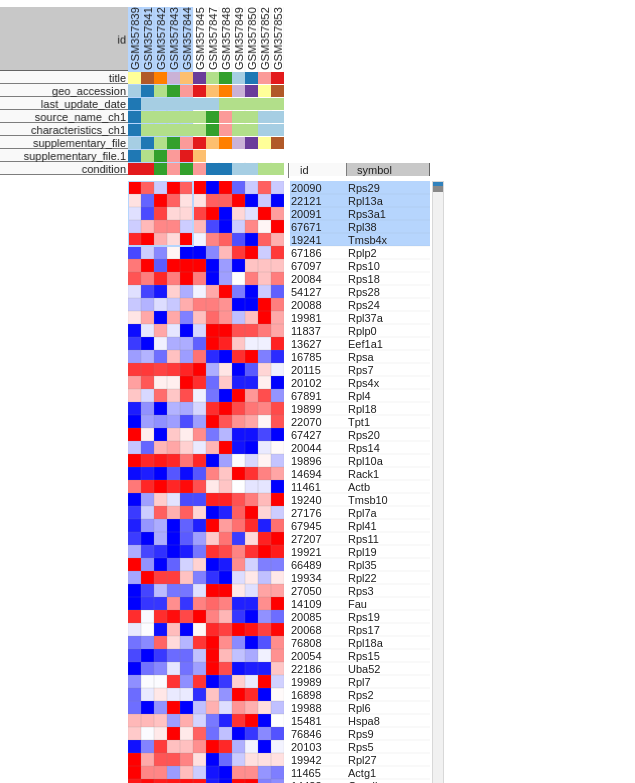
\includegraphics[scale=0.5]{heatmap14308.png}
  \caption{Визуализация матрицы GSE14308 в виде тепловой карты в веб-приложении Morpheus}
  \label{matrixvis}
\end{figure}


Также к основным методам анализа относятся:
\begin{itemize}
\item кластеризация:\begin{itemize}
\item иерархическая: метод упорядования данных таким образом, чтобы их можно было визуализировать в виде дерева (дендрограммы);
\item вероятностная: метод разбиения данных на несколько групп (кластеров);\end{itemize}
\item дифференциальная экспрессия: метод, позволяющий сравнивать поведение генов в разных условиях и искать закономерности;
\item метод главных компонент: метод для уменьшения размерности данных с наименьшей потерей информации. 
\end{itemize}

\section{Существующие решения для анализа экспрессии генов}
\subsection{R/Bioconductor}
\textbf{R} --- язык программирования для статистического анализа данных и работы с графикой~\cite{rproject}.

\textbf{Bioconductor} --- библиотека, содержащая в себе множество реализаций биоинформатических алгоритмов и методов обработки биологических данных на \emph{R}. Она постоянно обновляется, пополняется новыми библиотеками, модерируется сообществом~\cite{bioconductor}. \emph{R} и \emph{Bioconductor} очень популярны в биоинформатической среде ввиду предоставляемых возможностей.

Однако для качественного и полноценного анализа с помощью этих инструментов, нужно иметь навыки программирования на \emph{R}, что весьма неудобно для исследователей биологических специальностей.

\subsection{GENE-E}
\textbf{GENE-E} --- Платформа для анализа данных и визуального исследования данных, созданная на \emph{Java} и \emph{R}~\cite{genee}. Содержит в себе множество полезных для исследования инструментов: тепловые карты, кластеризацию, фильтрацию, построение графиков и т.д. Позволяет исследовать любые данные в виде матрицы. К тому же, содержит дополнительные инструменты для данных генетической экспрессии.

Недостатки:
\begin{itemize}
\item чтобы использовать, необходимо устанавливать на свой компьютер;
\item поддержка данного приложения прекратилась в связи с созданием \emph{morpheus.js}~\cite{morpheus};
\item не имеет открытого исходного кода, а только \emph{API} для взаимодействия и создания новых приложений на его основе.
\end{itemize}

\subsection{morpheus.js}
\textbf{Morpheus.js} --- веб-приложение для визуализации и анализа матриц от создателя \emph{GENE-E}~\cite{morpheus}. В отличие от предшественника, создано на \emph{JavaScript} и с открытым исходным кодом. Удобно для использования исследователями без навыков программирования и так же, как и \emph{GENE-E}, применимо к любым матрицам.

Недостатки:
\begin{itemize}
\item ограниченный набор функций, которых недостаточно для полноценного анализа;
\item для расширения биоинформатическими алгоритмами, не прибегая к дополнительным инструментам, требуется реализовывать их заново на \emph{JavaScript};
\end{itemize}

\subsection{ProjectX}
\textbf{ProjectX} --- веб-приложение, созданное в рамках выпускной квалификационной работы~\cite{projectx}, которое соединяло в себе возможности, предоставляемые \emph{API} \emph{GENE-E} и методы из библиотеки \emph{Bioconductor} с помощью \emph{OpenCPU}. Реализовано было данное приложение во фреймворке \emph{Django}. Преимуществом данного приложения перед \emph{GENE-E} была вопроизводимость исследований (на каждом этапе пользователь мог скачать исполняемый \emph{R}-код, эквивалентный коду, выполненному в сервисе), также он содержал в себе большее число методов анализа и обработки данных.

Недостатки:
\begin{itemize}
\item проект использовал в своей базе приложение, которое больше не поддерживается разработчиками;
\item работа над проектом была завершена до того, как у него появились пользователи, так что оно осталось невостребованным.
\end{itemize}

\section{Инструменты, которые могут быть применены}
\subsection{Язык R и библиотека Bioconductor}
Как было сказано ранее, \emph{Bioconductor} полон актуальными и широко используемыми биоинформатическими алгоритмами, в том числе и для анализа экспрессии генов. Соответственно, реализовывать их заново обычно нет необходимости и можно использовать их для достижения целей этой работы.

\subsection{JavaScript и Node.js}
\textbf{JavaScript} --- мультипарадигменный скриптовый язык программирования, широко используемый для создания веб-приложений.

\textbf{Node.js} --- программная платформа, превращающая JavaScript в язык общего назначения, добавляя возможность взаимодействовать с устройствами ввода-вывода, использовать внешние библиотеки, написанные на других языках. В основе Node.js лежит событийно-ориентированное и асинхронное программирование с неблокирующим вводом-выводом.~\cite{nodejs}

\subsection{R shiny}
\subsection{OpenCPU}
\textbf{HTTP} (\emph{HyperText Transfer Protocol}) ---  протокол прикладного уровня передачи данных на основе технологии <<клиент-сервер>>~\cite{http}.

\textbf{HTTP API} - набор процедур и функций, вызов которых и возвращение их результа осуществляется посредством протокола \emph{HTTP}.

\textbf{RPC} (\emph{Remote Procedure Call}) --- класс технологий, позволяющих компьютерным программам вызывать функции или процедуры в другом адресном пространстве.

\textbf{Веб-сервер} --- сервер, принимающий \emph{HTTP}-запросы от клиентов, обычно веб-браузеров, и выдающий им \emph{HTTP}-ответы.

\textbf{OpenCPU} --- система для встроенных научных вычислений и воспроизводимых исследований, предоставляющая \emph{HTTP API} для вызова R-функций и взаимодействия с R-объектами с помощью \texttt{POST} и \texttt{GET} запросов~\cite{opencpu}.

\subsubsection{OpenCPU-сервер}
\emph{OpenCPU}-сервер можно запустить одним из следующих способов:
\begin{itemize}
\item однопользовательский сервер: сервер запускается из активной \emph{R}-сессии и предназначен в основном для разработки и локального использования. Такой сервер не поддерживает параллельных запросов, так как \emph{R}-сессии работают в одном потоке;
\item облачный сервер: этот сервер можно запустить на \emph{Ubuntu 16.04} и выше. Запуск и настройка облачного сервера осуществляется с помощью \emph{apache} или \emph{nginx}. В отличие от однопользовательского сервера, здесь поддерживаются параллельные запросы и настройка безопасности.
\end{itemize}

\subsubsection{OpenCPU API}
Входной точкой \emph{API} является \texttt{/ocpu/}.
\texttt{GET}-запрос используется для получения некоторого ресурса, а \texttt{POST}-запрос используется для \emph{RPC}. На таблице~\ref{ocpu_api} можно увидеть более подробное описание запросов.

\begin{table}[!h]
  \small
\caption{Запросы к \emph{OpenCPU}-серверу, их аргументы и действия}\label{ocpu_api}
\centering
\begin{tabu}{|l|L|K|l|}
  \hline
Запрос        & Действие          & Аргументы                    & Пример                                 \\\hline 
\texttt{GET}  & посмотреть объект & формат представления объекта & GET /ocpu/library/MASS/R/cats/json     \\\hline
\texttt{POST} & вызвать функцию   & аргументы функции            & POST /ocpu/library/stats/R/rnorm       \\\hline
\texttt{GET}  & прочитать файл    & -                            & GET /ocpu/library/MASS/NEWS            \\\hline
\texttt{POST} & запустить скрипт  & аргументы запуска скрипта    & POST /ocpu/library/MASS?scripts/ch01.R \\\hline
\end{tabu}
\end{table}

На \emph{OpenCPU}-сервере могут быть доступны:
\begin{itemize}
\item библиотеки и содержащиеся в них пакеты: \texttt{/ocpu/library/{pkgname}/};
\item пакеты из \emph{git}-репозиториев: \texttt{/ocpu/apps/{gituser}/{reponame}/};
\item пакеты, установленные в домашней директории \emph{Linux}-пользователя: \texttt{/ocpu/user/{username}/library/{pkgname}/};
\item временные сессии, содержащие вывод от запуска функции или скрипта: \texttt{/ocpu/tmp/{key}/}.
\end{itemize}

\subsubsection{Opencpu.js}
Так как зачастую \emph{OpenCPU} используется разработчиками для использования \emph{R} в веб-приложениях для анализа и визуализации данных, для удобной интеграции \emph{JavaScript} и \emph{R} существует библиотека \textit{opencpu.js}, которая реалазует \emph{RPC}-вызовы по принципу \emph{Asynchronous JavaScript and XML} (\emph{Ajax}~\cite{ajax}). Таким образом запросы обрабатываются в фоновом режиме, тем самым не замедляя работу графического интерфейса и вычислений, осуществляемых на стороне клиента.

В данной библиотеке реализован класс \texttt{Session}, содержащий в себе ключ сессии, адреса на ссылки, файлы и переменные, существующие внутри сессии.

Для подключения к \emph{R}-пакету на \emph{OpenCPU}-сервере удобно использовать код, представленный на листинге~\ref{connect}. Для успешного подключения \emph{R}-пакет должен быть предварительно установлен на \emph{host}-машину, на которой располагается сервер. 

\begin{lstlisting}[float=!h,caption={Подключение к \emph{R}-пакету},label={connect}]
  ocpu.seturl("//hostname/ocpu/library/{pkgname}/R");
\end{lstlisting}
После этого можно вызывать и запускать функции, содержащиеся в данном \emph{R}-пакете, например, как в листинге~\ref{call.example}.

\begin{lstlisting}[float=!h,caption={Шаблон вызова \emph{R}-функции из \emph{JavaScript}},label={call.example},language=JavaScript]
  var req = ocpu.rpc("function.name", arguments, callback(session) {
    \\ Handling result
  });
\end{lstlisting}

\subsection{Gene Expression Omnibus}
\textbf{Gene Expression Omnibus (GEO)} --- международный публичный репозиторий, агрегирующий и распространяющий различные формы геномных данных от исследовательского сообщества~\cite{geo}.

\emph{GEO} предоставляет устойчивую базу данных для эффективного хранения геномных данных, содержит их в качественно аннотированном формате и дает возможность удобно как добавлять новые данные для публикации, так и запрашивать интересующие данные для исследований.

В \emph{GEO} содержатся следующие типы и форматы данных:
\begin{itemize}
\item информация о платформе, на которой производилось секвенирование генов (\emph{Platform records}): \texttt{GPLxxx};
\item информация об образцах и условиях, в которых производились исследования этих образцов (\emph{Sample records}): \texttt{GSMxxx};
\item информация о непосредственно исследованиях, полученные данные и выводы (\emph{Series records}): \texttt{GSExxx}.
\item обработанная и подготовленная для дальнейшего статистического анализа \emph{GEO}-кураторами информация об исследованиях (\emph(DataSet records)): \texttt{GDSxxx}.
\end{itemize}

В библиотеке \emph{Bioconductor} есть \emph{R}-пакет \emph{GEOquery} для удобной загрузки данных из \emph{GEO}~\cite{geoquery}.

\subsection{Docker}
\textbf{Docker} --- программное обеспечение для автоматизации запуска и внедрения приложений внутри контейнеров~\cite{docker}.

Для дальнейшего описания данного инструмента введем несколько определений.

\textit{Образ} --- отдельный исполняемый пакет, включающий себя все необходимое для запуска единицы программного обеспечения, в том числе исходный код, библиотеки, переменные окружения, конфигурационные файлы. Зачастую образ построен на основе другого образа с дополнительной конфигураций. Образ компилируется по \textit{Dockerfile}, каждая команда в котором соответствует новому слою. При перекомпиляции обновляются только те слои, которые изменились. 

\textit{Контейнер} --- запущенный экземпляр образа. Контейнер обычно исполняется изолированно от окружения, имея доступ к файлам или портам хост-системы только при наличии соответствующей конфигурации.

В отличие от виртуальных машин, которые запускают гостевую операционную систему в каждом экземпляре, контейнеры могут разделять общее ядро, и вся информация, которая должна быть в контейнере, это исполняемый процесс и его зависимости. Исполняемые процессы из контейнеров работают как нативные процессы, и могут управляться по отдельности. 

Для контроля версий и хранения образов в открытом доступе используется \emph{Docker Hub}~\cite{dhub}. В этом хранилище можно как добавлять репозитории, управляемые вручную, так и поддерживать автоматические сборки (\textit{Automated Build}), которые привязаны к репозиториям на в популярных системах контроля версий: GitHub \cite{github} и Bitbucket \cite{bitbucket}.

\subsection{JSON}
\textbf{JSON} --- текстовый формат представления данных, основанный на \emph{JavaScript}, который, среди прочих достоинств, легко читается человеком~\cite{json}.

\emph{JSON}-текст представляет собой одну из следущих структур:\begin{itemize}
\item пара \textit{ключ}: \textit{значение}, где ключом может быть только регистрозависимая строка, а в качестве значения может выступата массив, число, строка, литералы или другой \emph{JSON}-объект;
\item набор значений.
\end{itemize}

\subsection{Protocol Buffers}
\textbf{Protocol Buffers (Protobuf)} --- гибкий, универсальный и автоматизированный механизм для сериализации структурированных данных~\cite{protobuf}.

Структура информации задается с помощью \texttt{*.proto}-файлов в форме сообщений (\texttt{message}).

\emph{ProtoBuf}-формат не является человекочитаемым, данные хранятся в двоичном формате. Для десериализации и дальнейшего чтения необходим соответствующий \texttt{*.proto}-файл. Файл с форматом компилируется соответствующим выбранному языку программирования компилятором, таким образом будет создан класс доступа к данным. С помощью этого класса уже можно сериализовать/десериализовать данные, получать данные с помощью \texttt{get}/\texttt{set}-методов и пр.

\subsection{Apache}
\textbf{Apache HTTP Server Project} --- устойчивый, полностью открытый \emph{HTTP}-сервер~\cite{apache}.
\subsection{HTML}

\section{Постановка задачи}
Рассмотрев существующие решения для анализа экспрессии генов и инструментов, которые могли бы пригодиться для будущих решений, можно сформулировать цель и основные задачи данной работы

\subsection{Цель работы}
Создать веб-приложение, интегрирующее существующие возможности веб-приложения morpheus.js и методы анализа, реализованные в Bioconductor.

\subsection{Основные задачи}
\begin{enumerate}
\item Разработать способ взаимодействия между js-клиентом и R и встроить его в morpheus.js, чтобы избежать реализации с нуля уже существующих алгоритмов;
\item Реализовать графический интерфейс в js-клиенте и серверную реализацию в R-пакете;
\item Соединить все составляющие в одном веб-приложении phantasus;
\item Запустить веб-приложение в открытый доступ для исследователей.
\end{enumerate}

\subsection{Требования к веб-приложению phantasus}
\subsubsection{Доступность}
Необходимо, чтобы веб-приложение phantasus было доступно для исследователей независимо от их местоположения и времени суток. Варианты действий:

\begin{enumerate}
\item Сделать его доступным по определенному веб-адресу, и тогда пользователь сможет продолжать исследования из любой точки, где есть подключение к интернету;
\item Предоставить возможность запускать приложение локально, например, с помощью Docker или внутри R.
\end{enumerate}

\subsubsection{Возможность дальнейшего расширения функционала}
Как уже было сказано выше, библиотека Bioconductor постоянно обновляется и пополняется новыми алгоритмами, а исследователи находят новые методы для анализа экспрессии генов, так что необходимо не только реализовать дополнительные методы, но также отладить и описать алгоритм действий для добавления новых.

\chapterconclusion
В данной главе были введены понятия биоинформатики и анализа экспрессии генов, обозначена цель работы и задачи, выполнение которых необходимо для ее достижения, представлены существующие решения с их достоинствами и недостатками, а также перечислен ряд инструментов, которые могут быть использованы для решения поставленных задач работы.

\chapter{Архитектура проекта phantasus}
В этой главе будут подробно рассмотрены следующие составляющие проекта:
\begin{itemize}
\item исходное веб-приложение \emph{Morpheus} (\emph{morpheus.js}), содержащиеся в нем методы и классы, которые будут необходимы для дальнейших модификаций;
\item созданный и использующися на серверной стороне проекта \emph{R}-пакет \emph{phantasus};
\item \emph{OpenCPU} как связь между модифицированным \emph{Morpheus} (\emph{phantasus.js}) на стороне клиента и \emph{R}-пакетом \emph{phantasus} на стороне сервера.
\end{itemize}
Также будут описаны сопутствующие инструменты и их предназначение в системе, и ключевые для архитектуры выдержки из исходного кода.

\section{morpheus.js}
Как уже было рассказано в обзоре, \emph{Morpheus} --- веб-приложение, полностью созданное на \emph{JavaScript}, для визуализации и анализа матриц.

В этом разделе будут описаны основные классы и функции, реализованные в исходном коде \emph{morpheus.js}, которые будут в дальнейшем необходимы для расширения функционала.

\subsection{Чтение данных}
В \emph{morpheus.js} данные могут быть загружены из файла одним из следующих путей:
\begin{itemize}
\item Из компьютера;
\item По \emph{URL}-ссылке;
\item Из \emph{Dropbox}.
\end{itemize}

Допустимые форматы загружаемых файлов:
\begin{itemize}
\item \emph{txt}-файл с \emph{tab}-разделителями;
\item \emph{Excel}-таблица;
\item \emph{Mutation Annotation Format} (\emph{MAF})~\cite{maf};
\item \emph{Gene Cluster Text} (\emph{GCT})~\cite{gct};
\item \emph{Gene Matrix Transposed} (\emph{GMT})~\cite{gmt}.
\end{itemize}

Для каждого формата файла в исходном коде morpheus.js присутствует соответствующий обработчик данных.

Также, \emph{morpheus.js} предлагает набор предзагруженных данных из базы \emph{The Cancer Genome Atlas} (\emph{TCGA})~\cite{tcga}.

\subsection{Класс Dataset}
Одним из ключевых классов всего веб-приложения является класс \texttt{Dataset}. В каждом экземпляре этого класса хранится вся необходимая информация о данных, в которую входят:

\begin{itemize}
\item числовая матрица, характеризующая уровень экспрессии всех генов во всех образцах;
\item количество строк и столбцов в матрице;
\item аннотация к образцам, например:\begin{itemize}
\item пол, возраст, контактную информацию испытуемых, если образцы были взяты с людей;
\item есть или нет инфекция в данном образце;
    \item способ лечения;
    \item  контакты ответственного за взятие данного образца и пр.;\end{itemize}
\item аннотация к генам, например:\begin{itemize}
    \item идентификатор гена в том или ином стандарте;
    \item числовые характеристики гена (средний уровень экспрессии по образцам, номер кластера) и пр.\end{itemize}
\end{itemize}

Аннотация реализована в классе \texttt{MetadataModel}, который представляет собой не что иное, как набор именованных векторов с характеристиками. В каждом векторе хранятся:

\begin{itemize}
\item название;
\item формат (строка, число);
\item массив значений.
\end{itemize}

Для векторов так же предусмотрены утилиты для визуализации. Так, например, есть возможность показать аннотацию в виде текста и/или цветом, что удобно для категориальных характеристик. 

\subsection{Класс SlicedDatasetView}
Чаще всего во время работы программы экземпляры класса \texttt{Dataset} становятся обернуты в оболочку из \texttt{SlicedDatasetView}. Этот дополнительный класс дает возможность не пересоздавать каждый раз \texttt{Dataset}, а просто добавляет к данным информацию о том, какие индексы строк и столбцов выбраны и используются в данный момент и в каком порядке.

\subsection{Класс HeatMap}
Данный класс предназначен для визуализации данных, обернутых в класс \texttt{Dataset} или \texttt{SlicedDatasetView}. Он дает возможность выбирать, какая аннотация будет представлена на экране, цветовой код, выбирать строки и столбцы, с которыми будут работать те или иные инструменты.

\subsection{Реализованные методы}
В \emph{morpheus.js} имеются реализации следующих методов обработки и анализа данных:

\begin{itemize}
\item \texttt{Adjust} --- инструмент для корректировки данных:\begin{itemize}
    \item $\log_{2}$;
    \item $\log_{2}^{-1}$;
    \item Квантиль-нормализация;
    \item Z-тест;
    \item Устойчивый Z-тест;\end{itemize}
\item \texttt{Collapse} --- инструмент, позволяющий агрегировать строки или столбцы с одинаковыми значениями с помощью функции: $\min$, $\max$, $mean$, $median$, $sum$, максимум 25-го и 75-го перцентилей;
\item \texttt{CalculatedAnnotation} --- добавление вычисленной аннотации для строк или столбцов;
\item \texttt{Similarity Matrix} --- построение матрицы соответствия строк или столбцов друг другу;
\item \texttt{Transpose} --- транспонирование матрицы;
\item \texttt{t-SNE} --- реализация алгоритма снижения размерности;
\item \texttt{ChartTool} --- построение графиков.
\end{itemize}

Также присутствуют фильтрация и сортировка.

\subsection{Класс DatasetUtil}
Класс \texttt{DatasetUtil} содержит в себе утилиты для обработки и чтения данных в \texttt{Dataset}:\begin{itemize}
\item обработка входных файлов с данными и отправка их на соответствующий класс чтения в зависимости от формата;
\item поиск по данным;
\item преобразование данных в \emph{JSON} и обратно.
\end{itemize}

\section{phantasus.js}
В этом разделе будет рассмотрен модифицированный вариант \emph{morpheus.js} и потребовавшиеся для его расширения компоненты.

\subsection{Поддержка Protocol Buffers --- protobuf.js}
Чаще всего размеры обрабатываемых матриц 10000-40000 строк на 12-40 столбцов. Соответственно, пересылать их между клиентом и сервером в \emph{JSON}-формате слишком долго.

Как было сказано в обзоре, технология \emph{Protocol Buffers} позволяет лучше сериализовать данные, чтобы уменьшить размер пересылаемого пакета.

К сожалению, \emph{Google Developers} официально поддерживают только \emph{Java}, \emph{Python}, \emph{C++}, \emph{Go}, \emph{Objective-C}, \emph{Ruby}, \emph{JavaNano} и \emph{C\#}. Для \emph{JavaScript} сообщество создает поддержку самостоятельно. После анализа существующих решений, было решено выбрать библиотеку \emph{ProtoBuf.js}~\cite{protobufjs}.

С помощью класса \texttt{Builder}, который компилируется из \texttt{*.proto}-файлов и позволяет получить доступ к сериализованным данным, можно закодировать соответствующий \emph{JSON}-объект в \texttt{Uint8Array}, чтобы после пересылать его в сжатом виде на сервер.

Для преобразования объекты классов \texttt{Dataset} и \texttt{SlicedDatasetView} в сериализованнный \texttt{Uint8Array} с помощью протокола описанного в приложении~\ref{proto}. Соответственно, предварительно данные из \texttt{Dataset} с помощью добавленных в \texttt{DatasetUtil} методов преобразовываются в соответствующий \emph{JSON}-объект, а после с помощью \texttt{Builder} сериализуется.

\subsection{Клиентская сторона OpenCPU --- opencpu.js}
В обзоре было рассказано об \emph{OpenCPU} и его полезных свойствах. В данной работе он нужен для связи \emph{JavaScript}-клиента и \emph{R}-сервера.


\subsection{Интерактивные графики --- plotly.js}
Для отображения интерактивных графиков используется библиотека \emph{plotly.js}\cite{plotly}, которая предоставляет удобное API, в котором описание графика строится в JSON-формате. Соответственно, вся графическая работа лежит на клиенте.

\subsection{Поддержка ExpressionSet}
В phantasus.js в Dataset добавлено дополнительное поле esSession, в котором находится объект класса Promise для асинхронного обновления ключа сессии в этом поле.

При загрузке или обновлении Dataset осуществляется следующий ряд действий:
\begin{enumerate}
\item В поле dataset.esSession записывается экземпляр класса Promise, который позволяет продолжать загрузку данных в фоновом режиме, а также ждать, когда данные будут обработаны прежде чем запускать функции использующие ExpressionSet в качестве аргумента (pcaPlot, kmeans, limma). При создании Promise в аргументах указывается две функции: \texttt{reject} и \texttt{resolve};
\item Актуальное содержимое экземпляра класса Dataset вместе с матрицей и аннотацией сериализуется в ProtoBuf по протоколу, описанному в приложении \ref{proto};
\item С помощью opencpu.js отправляется RPC за функцией \texttt{createES} с аргументом в виде сериализованных данных;
\item Данные поступают на сервер, десериализуются там автоматически и функция \texttt{createES} создает ExpressionSet, являющийся копией Dataset из клиента;
\item Функция \texttt{createES} объявляет данный ExpressionSet глобальной переменной, таким образом имеется доступ к этому объекту по API-entrypoint \texttt{/ocpu/tmp/{key}/R/es};
\item По завершении RPC получает ключ временной сессии, содержащий созданный ExpressionSet и завершает Promise с \texttt{resolve(session)};
\item Если во время одного из этапов произошла ошибка, то Promise завершается с \texttt{reject(error)} с текстом ошибки.
\end{enumerate}

\subsection{Инструмент PcaPlotTool}
Данный инструмент предназначен для построения графиков в соответствие с методом главных компонент.
В качестве аргументов на вход к инструменту подается:
\begin{itemize}
\item Номера образцов для сравнения;
\item Категориальная аннотация для различения точек по цвету (если не указана, то стандартный цвет);
\item Числовая аннотация для различения точек по размеру (если не указана, то стандартный размер);
\item Аннотация для подписей к точкам (если не указана, то без подписи);
\item Функция замены NA в данных при вычислении матрицы PCA (mean или median).
\end{itemize}

На сервер отправляется только ключ сессии и функция замены, содержащей актуальный ExpressionSet. После чего на клиент возвращается матрица PCA, по которой уже на клиенте отрисовывается интерактивный график с учетом графических аргументов в PcaPlot.

\subsection{Инструмент KmeansTool}
На клиенте в инструменте KmeansTool осуществляется только сбор значений аргументов:
\begin{itemize}
\item Количество кластеров, на которые нужно разбить данные;
\item Функция замены NA в данных.
\end{itemize}

Данные аргументы и ключ сессии актуального ExpressionSet отправляются на сервер, после чего, получив список Ген-Номер кластера на клиенте отрисовывается новая аннотация к строкам.

\subsection{Инструмент LimmaTool}
На клиенте осуществляется получение аргументов:
\begin{itemize}
\item Какие аннотации образцов участвуют в сравнении;
\item Какая комбинация значений указанных выше аннотаций обозначает класс A;
\item Аналогично для класса B.
\end{itemize}

После чего образцы разбиваются на классы A и B, либо обозначаются пустыми, в соответствии с полученными аргументами. Список Образец-Класс и ключ сессии актуального ExpressionSet после отправляются на сервер, где происходит вычисление.
От сервера приходит файл с сериализованной матрицей результатов, которые с помощью protobuf.js разбираются и отрисовываются в виде аннотации к строкам.

\section{R-пакет phantasus}
Весь реализованный функционал должен иметь клиентскую часть в виде графического интерфейса и серверную в виде R-функции.
Прежде чем рассматривать созданные функции, будут представлены имеющиеся необходимые элементы.

\subsection{Biobase и ExpressionSet}
Необходимый минимум функций для работы с геномными данными содержится в R-пакете Biobase \cite{biobase}.

Класс ExpressionSet \cite{expressionset} так же содержится в Biobase. Он помогает представлять данные об экспрессии генов в удобном формате:
\begin{itemize}
\item assayData --- описание матрицы:\begin{itemize}
\item features --- количество генов;
\item samples --- количество образцов;
\item exprs --- числовая матрица экспрессии; \end{itemize}
\item phenoData --- аннотация к образцам:\begin{itemize}
\item sampleNames --- идентификаторы образцов;
\item varLabels --- названия характеристик;
\item varMetadata --- описание характеристик;
\item pData --- матрица характеристик;\end{itemize}
\item featureData --- аннотация к генам:\begin{itemize}
\item featureNames --- идентификаторы генов;
\item fvarLabels --- названия характеристик;
\item fvarMetadata --- описание характеристик;
\item fData --- матрица характеристик.\end{itemize}
\end{itemize}

Для доступа к каждому из элементов есть одноименная функция, что позволяет удобно взаимодействовать с экземплярами класса. Также многие из функций обработки данных в Bioconductor и в Biobase в частности завязаны на использование ExpressionSet.

Все реализованные в R-пакете phantasus функции принимают на вход в качестве одного из аргументов экземпляр класса ExpressionSet.

\subsection{Поддержка Protocol Buffers --- protolite}
Поддержка ProtoBuf cо стороны R-сервера осуществляется с помощью R-пакета protolite \cite{protolite}. В реализованных функциях данный пакет используется каждый раз, когда необходимо вернуть матрицу больших размеров. Вместо отправки ее в исходном виде или в JSON предпочтительнее сериализовать результат и сохранить в файл, который после будет прочитан на клиенте.

\subsection{Создание ExpressionSet из данных}
В начале работы с phantasus необходимо загрузить данные. Если данные загружены из файла, то они будут сначала обработаны на клиенте, а после пересланы на сервер для создания ExpressionSet из них с помощью кода на листинге~\ref{createES}

\begin{lstlisting}[float=!h,caption={Функция создания ExpressionSet из исходных данных},label={createES},language=R]
createES <- function(data, pData, varLabels, fData, fvarLabels) {
  exprs <- t(data)
  phenoData <- AnnotatedDataFrame(data.frame(pData))
  varLabels(phenoData) <- varLabels
  
  featureData <- AnnotatedDataFrame(data.frame(fData))
  varLabels(featureData) <- fvarLabels
 
  es <- ExpressionSet(assayData = exprs, phenoData=phenoData, featureData = featureData)
  assign("es", es, envir = parent.frame())
  es
}
\end{lstlisting}

По завершении функция отправляет \texttt{es} в глобальные переменные, чтобы ExpressionSet был доступен по адресу: /ocpu/tmp/session-key/R/es. Таким образом, получив ключ данной сессии, можно иметь доступ и к ExpressionSet, находящемуся в ней.

Ключ сессии обновляется каждый раз при изменении Dataset в phantasus.js (Adjust, Collapse, new HeatMap, Transpose). Изменные данные пересылаются на сервер и ключ сессии обновляется в поле esSession в Dataset.
\subsection{Загрузка данных из GEO --- loadGEO}
В обзоре были описаны форматы данных в репозитории Gene Expression Omnibus.
В phantasus загрузка данных из GEO осуществляется следующим образом:
\begin{enumerate}
\item Функция loadGEO принимает на вход идентификатор GEO;
\item В зависимости от его вида (GSE или GDS) запускаются дополнительные функции (getGSE на листинге~\ref{getGSE} и getGDS на листинге~\ref{getGDS});
\item После с помощью \texttt{GEOquery::getGEO} загружаются данные с аннотацией (или подгружаются из кэша, если их уже загружали);
\item Результат обрабатывается, создается ExpressionSet и отправляется в глобальные переменные;
\item В файл записываются сериализованные в ProtoBuf данные, которые после считает и обработает клиент
\end{enumerate}
\begin{lstlisting}[float=!h,caption={Загрузка данных типа GSE из Gene Expression Omnibus},label={getGSE},language=R]
getGSE <- function(name, destdir = tempdir()) {
  es <- getGEO(name, AnnotGPL = T, destdir = destdir)[[1]]
  featureData(es) <- featureData(es)[,grepl("symbol", fvarLabels(es), ignore.case = T)]
  phenoData(es) <- phenoData(es)[,grepl("characteristics", varLabels(es), ignore.case = T)
                                  | (varLabels(es) %in% c("title", "id", "geo_accession"))]
  chr <- varLabels(es)[grepl("characteristics", varLabels(es), ignore.case = T)]
  take <- function(x, n) {
    sapply(x, function(x) { x[[n]] })
  }
  rename <- function(prevName, x) {
    splitted <- strsplit(x, ": ")
    sumlength <- sum(sapply(as.vector(splitted), length))
    if (sumlength != 2 * length(x)) {
       return(list(name = prevName, x = x))
    }
    splittedFirst <- unique(take(splitted, 1))
    if (length(splittedFirst) == 1) {
       res = list(name = splittedFirst[1], x = take(splitted, 2))
    }
    else {
       res = list(name = prevName, x = x)
    }
    res
  }
  renamed <- lapply(chr, function(x) { rename(x, as.vector(pData(es)[,x])) })
  phenoData(es) <- phenoData(es)[, !(varLabels(es) %in% chr)]
  pData(es)[,take(renamed,1)] <- take(renamed,2)
  es
}
\end{lstlisting}

\begin{lstlisting}[float=!h,caption={Загрузка данных типа GDS из Gene Expression Omnibus},label={getGDS},language=R]
 getGDS <- function(name, destdir = tempdir()) {
  l <- getGEO(name, destdir = destdir)
  table <- slot(l, 'dataTable') # extracting all useful information on dataset
  data <- Table(table)  # extracting table ID_REF | IDENTIFIER/SAMPLE | SAMPLE1 | ...
  columnsMeta <- Columns(table) # phenoData
  sampleNames <- as.vector(columnsMeta[["sample"]])
  rownames <- as.vector(data[["ID_REF"]])
  symbol <- as.vector(data[["IDENTIFIER"]])
  data <- data[,sampleNames] # expression data
  exprs <- as.matrix(data)
  row.names(exprs) <- rownames
  row.names(columnsMeta) <- sampleNames
  # columnsMeta <- columnsMeta[,!(colnames(columnsMeta) %in% c('sample'))] 
  pData <- AnnotatedDataFrame(data.frame(columnsMeta, check.names = F))
  fData <- data.frame(matrix(symbol, nrow(exprs), 1));
  colnames(fData) <- "symbol"
  fData <- AnnotatedDataFrame(fData)
  featureNames(fData) <- rownames
  ExpressionSet(assayData = exprs, phenoData = pData, featureData = fData)
}
\end{lstlisting}

Код и его дополнительные рутины можно увидеть на листинге~\ref{loadGEO}.

\begin{lstlisting}[float=!h,caption={Загрузка данных из Gene Expression Omnibus},label={loadGEO},language=R]
loadGEO <- function(name, type = NA) {
  es <- getES(name, type, destdir = "/var/phantasus/cache")
  assign("es", es, envir = parent.frame())
  data <- as.matrix(exprs(es)); colnames(data) <- NULL; row.names(data) <- NULL

  pdata <- as.matrix(pData(es)); colnames(pdata) <- NULL; row.names(pdata) <- NULL

  participants <- colnames(es)
  rownames <- rownames(es)

  fdata <- as.matrix(fData(es))
  colnames(fdata) <- NULL
  row.names(fdata) <- NULL

  res <- list(data = data, pdata = pdata,
              fdata = fdata, rownames = rownames,
              colMetaNames = varLabels(phenoData(es)),
              rowMetaNames = varLabels(featureData(es)))

  f <- tempfile(pattern = "gse", tmpdir = getwd(), fileext = ".bin")
  writeBin(protolite::serialize_pb(res), f)
  f
}
getES <- function(name, type = NA, destdir = tempdir()) {
  if (is.na(type)) {
     type = substr(name, 1, 3)
  }
  if (type == 'GSE') {
    es <- getGSE(name, destdir)
  }
  else if (type == 'GDS') {
    es <- getGDS(name, destdir)
  }
  else {
    stop("Incorrect name or type of the dataset")
  }
  es
}
\end{lstlisting}

\subsection{Дифференциальная экспрессия --- limmaAnalysis}
R-пакет limma \cite{limma} предоставляет методы для вычисления дифференциальной экспрессии. Данная функция помогает увидеть, насколько случайны или нет различия между образцами в генах в разных условиях.

Соответственно, было решено включить в phantasus поддержку такой функции.

Реализация функции \texttt{limmaAnalysis} в R-пакете phantasus принимает в себя ExpressionSet и вектор с соответствием Образец-Класс. Класс в этом векторе может быть A, B или пустым. Необходимо сравнить классы A и B, а для этого нужно дополнить фенотипические данные ExpressionSet полученным вектором.
После дизайн сравнения передается в функцию, которая возвращает матрицу статистических характеристик к каждому гену.
Эта матрица далее сериализуется в ProtoBuf, записывается в файл, который будет в дальнейшем разобран на клиенте.

Код функции \texttt{limmaAnalysis} представлен на листинге~\ref{limmaAnalysis}.

\begin{lstlisting}[float=!h,caption={Реализация дифференциальной экспрессии в R-пакете phantasus},label={limmaAnalysis},language=R]
limmaAnalysis <- function(es, rows = c(), columns = c(), fieldValues) {
  assertthat::assert_that(length(columns) == length(fieldValues) || length(columns) == 0)
  rows <- getIndicesVector(rows, nrow(exprs(es)))
  columns <- getIndicesVector(columns, ncol(exprs(es)))
  fieldName <- "Comparison"
  fieldValues <- replace(fieldValues, fieldValues == '', NA)
  new.pdata <- pData(es)[columns,]
  new.pdata[[fieldName]] <- as.factor(fieldValues)
  new.pdata <- new.pdata[!is.na(new.pdata[[fieldName]]),]
  new.sampleNames <- row.names(new.pdata)
  es.copy <- es[rows, new.sampleNames]
  pData(es.copy) <- new.pdata
  fData(es.copy) <- data.frame(row.names=rownames(es.copy))
  es.design <- model.matrix(~0 + Comparison, data = pData(es.copy))
  colnames(es.design) <- gsub(pattern = fieldName,
                              replacement = '',
                              x = make.names(colnames(es.design)))
  fit <- lmFit(es.copy, es.design)
  fit2 <- contrasts.fit(fit, makeContrasts(B - A,
                                           levels=es.design))
  fit2 <- eBayes(fit2)
  de <- topTable(fit2, adjust.method="BH", number=Inf)
  de <- de[row.names(fData(es.copy)),]
  f <- tempfile(pattern = "de", tmpdir = getwd(), fileext = ".bin")
  writeBin(protolite::serialize_pb(as.list(de)), f)
  f
}
\end{lstlisting}

\subsection{Статистические функции --- stats}
R-пакет stats \cite{stats} содержит в себе большинство современных используемых методов статистического анализа.
В данной работе используются два: PCA (метод главных компонент) и kmeans (кластеризация).

\chapterconclusion
В данной главе были рассмотрены основные составляющие проекта:
\begin{itemize}
\item morpheus.js --- база для расширения, поэтому были описаны важные компоненты, с которыми необходимо взаимодействовать во время дополнения проекта новым функционалом;
\item phantasus.js --- расширенный morpheus.js. Были описаны дополнения: новые инструменты, поддержка ProtoBuf, поддержка актуального состояния ключа сессии ExpressionSet для каждого Dataset;
\item R-пакет phantasus --- R-пакет, содержащий в себе серверные реализации всех добавленных методов и инструментов.
\end{itemize}

\chapter{Реализация и использование}
\section{Структура git-репозитория}
Как следует из главы об архитектуре проекта, проект состоит из двух составляющих:
\begin{itemize}
\item phantasus.js --- fork репозитория morpheus.js \cite{morpheus};
\item phantasus --- репозиторий для R-пакета.
\end{itemize}
Внутри репозитория phantasus находится подмодуль для репозитория phantasus.js.
Соответственно, чтобы загрузить целиком весь проект достаточно вызвать команду из листинга~\ref{clonerepo}.
\begin{lstlisting}[float=!h,language=bash,label={clonerepo},caption={Клонирование репозитория проекта phantasus}]
  git clone --recursive https://github.com/ctlab/phantasus.git
\end{lstlisting}

\section{Кэш для данных из GEO}
Независимо от способа запуска, данные, загруженные из GEO, кэшируются в определенной папке, чтобы не было необходимости перескачивать их заново.

\section{Единый R-пакет phantasus}
Так как проект теперь существует в виде почти единого git-репозитория, его легко можно использовать как полноценный R-пакет, содержащий в себе в том числе и файлы для веб-приложения.
С помощью функции, представленной на листинге~\ref{serve.R}, можно запускать веб-приложение phantasus непосредственно из R.
\lstinputlisting[float=!h,language=R,label={serve.R},caption={Функция для запуска приложения из R}]{listings/serve.R}

\section{Docker-образ phantasus}
На hub.docker.com существует автоматический репозиторий, привязанный к git-репозиторию phantasus. Для каждой перекомпиляции он использует Dockerfile с листинга~\ref{dockerfile}, расположенный в репозитории.

На данный момент существуют две ветки Docker-образа:
\begin{itemize}
\item master --- компиляция происходит из master-веток составляющих проекта, чаще всего эти скомпилированные образы стабильны и отправляются в открытый доступ для использования;
\item develop --- компиляция происходит из develop-веток составляющих проекта, эти образы используются для тестирования всего приложения в целом, тестирования нового функционала и не предназначены для использования на серверах.
\end{itemize}

Чтобы загрузить Docker-образ, нужно воспользоваться командой с листинга~\ref{dockerpull}
\begin{lstlisting}[float=!h,language=bash,label={dockerpull},caption={Загрузка Docker-образа phantasus}]
  docker pull dzenkova/phantasus
\end{lstlisting}

\subsection{Запуск Docker-контейнера}

\section{Настройка с помощью Apache}
\subsection{Переадресация OpenCPU-сервера}
После того, как сравнили скорость работы с использованием single-user OpenCPU-сервера и multi-user, пришли к выводу, что скорость доступа к первому выше из-за того, что RApache работает достаточно медленно.

Соответственно, происходит переадресация запросов с /ocpu на //localhost:8001/ocpu.
\subsection{Балансировщик для multi-user соединения}
Из-за того, что используется single-user OpenCPU-сервер, несколько людей, использующих веб-приложение phantasus одновременно, вынуждены ждать, пока закончится запрос для одного.

Чтобы такого не происходило, запускается четыре экземпляра OpenCPU-сервера и с помощью Apache-балансировщика можно получать доступ к R-серверу параллельно.

\section{Статистика использования}

\chapterconclusion
В данной главе были рассмотрены технические подробности реализации веб-приложения: инструкции для запуска, варианты использования и подробности настройки веб-приложения на сервере.

%% Макрос для заключения. Совместим со старым стилевиком.
\startconclusionpage

\printmainbibliography

%% После этой команды chapter будет генерировать приложения, нумерованные русскими буквами.
%% \startappendices из старого стилевика будет делать то же самое
\appendix
\chapter{Протокол сериализации в ProtoBuf}
R-пакет protolite использует стандартный протокол сериализации, представленный на листинге~\ref{proto}. Этот же протокол было решено использовать и при сериализации на клиенте для однообразия и для корректного разбора сообщений как на клиенте от сервера, так и на сервере от клиента.
\lstinputlisting[float=!h,caption={Протокол сериализации R-пакета protolite},label={proto}]{listings/message.proto}
\chapter{Dockerfile}
\lstinputlisting[float=!h,caption={Dockerfile для Docker-образа веб-приложения phantasus},label={dockerfile}]{listings/Dockerfile}

\end{document}
